\documentclass[main.tex]{subfiles}
\graphicspath{{\subfix{img/}}}

\begin{document}

\chapter{Modelagem do quadricóptero}
\label{chap:modelagem}

\textcolor{red}{GRANDE MUDANÇA: tem mais sentido em começar do sistema em rotação não inercial (u,v,w) e fazer considerações de giroscópio e conversão para inercial e depois rotação para o sistema fixo.}

A modelagem dinâmica do voo de um quadricóptero relaciona as forças e momentos de seus atuadores com os deslocamentos e velocidades correspondentes do veículo. Para tanto, os balanços de força e de momento devem ser considerados em relação a um referencial não inercial \cite{classica:livro}, conforme a Equação: \ref{eq:revisao_coriolis}:

\begin{equation}\label{eq:revisao_coriolis}
    \begin{gathered}
        \boldsymbol{I}\dot{\boldsymbol{\omega}} + \boldsymbol{\omega}\times(\boldsymbol{I}\boldsymbol{\omega}) = \Sigma \boldsymbol{M}\\
        \boldsymbol{I} = \begin{bmatrix}
             I_{xx} & -I_{xy} & -I_{xz}\\
            -I_{xy} &  I_{yy} & -I_{yz}\\
            -I_{xz} & -I_{yz} & I_{zz}
        \end{bmatrix} \hspace{0.4cm},\hspace{0.4cm}
        \boldsymbol{\omega} = \begin{bmatrix}
            \omega_{x}\\
            \omega_{y}\\
            \omega_{z}
        \end{bmatrix} \hspace{0.4cm},\hspace{0.4cm}
        \Sigma\boldsymbol{M} = \begin{bmatrix}
            \Sigma M_{x}\\
            \Sigma M_{y}\\
            \Sigma M_{z}
        \end{bmatrix}
    \end{gathered}
\end{equation}

Onde $\boldsymbol{I}$ representa o tensor de inércia,  $\boldsymbol{\omega}$ a velocidade angular e $\boldsymbol{M}$ os momentos aplicados. Cabe observar que os produtos de inércia em geral são próximos de nulos. A equação anterior também pode ser representada na forma escalar, de forma a explicitar os efeitos dos momentos aplicados a cada eixo, conforme apresentado na Equação \ref{eq:revisao_coriolis_escalar}. 

\begin{align}\label{eq:revisao_coriolis_escalar}
    \begin{split}
        I_{xx}\dot{\omega}_{x} + (I_{zz} - I_{yy})\omega_y\omega_z &= \Sigma M_x\\
        I_{yy}\dot{\omega}_{y} + (I_{xx} - I_{zz})\omega_z\omega_x &= \Sigma M_y\\
        I_{zz}\dot{\omega}_{z} + (I_{yy} - I_{xx})\omega_x\omega_y &= \Sigma M_z
    \end{split}
\end{align}
e
Deve-se considerar também o torque que um atuador causa na estrutura devido ao movimento de precessão com relação à sua direção de aplicação, nomeado efeito giroscópico. Este torque é determinado pela Equação \ref{eq:gyro_vec}, em função dos vetores das velocidades angulares de precessão $(\boldsymbol{\omega_p})$ e dos momentos angulares gerados pelos propulsores $(\boldsymbol{\lambda})$.

\begin{equation}\label{eq:gyro_vec}
    \boldsymbol{\tau_{gyro}} = \boldsymbol{\omega_p}\times\boldsymbol{\lambda}
\end{equation}

As equações \ref{eq:gyro_vec} e \ref{eq:atitude_escalar_som} podem ser combinadas para definir a atitude do veículo. Considerando-se que o produto vetorial na direção vertical é nulo pelos vetores serem colineares, que o momento angular é dado pelo produto entre o momento de inércia de todas as hélices $I_r$ com a soma das suas velocidades angulares $\Omega$, e que estas mesmas velocidades são descritas conforme a nomenclatura definida na Tabela \ref{tab:angulos}, obtém-se:

\begin{equation}\label{eq:atitude_escalar_som}
    \begin{split}
        I_{xx}\dot{p} &= (I_{zz} - I_{yy})qr + I_r\Omega q + \Sigma M_x\\
        I_{yy}\dot{q} &= (I_{xx} - I_{zz})pr - I_r\Omega p + \Sigma M_y\\
        I_{zz}\dot{r} &= (I_{yy} - I_{xx})pq + \Sigma M_z
    \end{split}
\end{equation}

\begin{figure}[!h]
    \centering
    \caption{Simbologia da atitude de um quadricóptero com eixos orientados x, y e z em vermelho, verde e azul respectivamente.}
    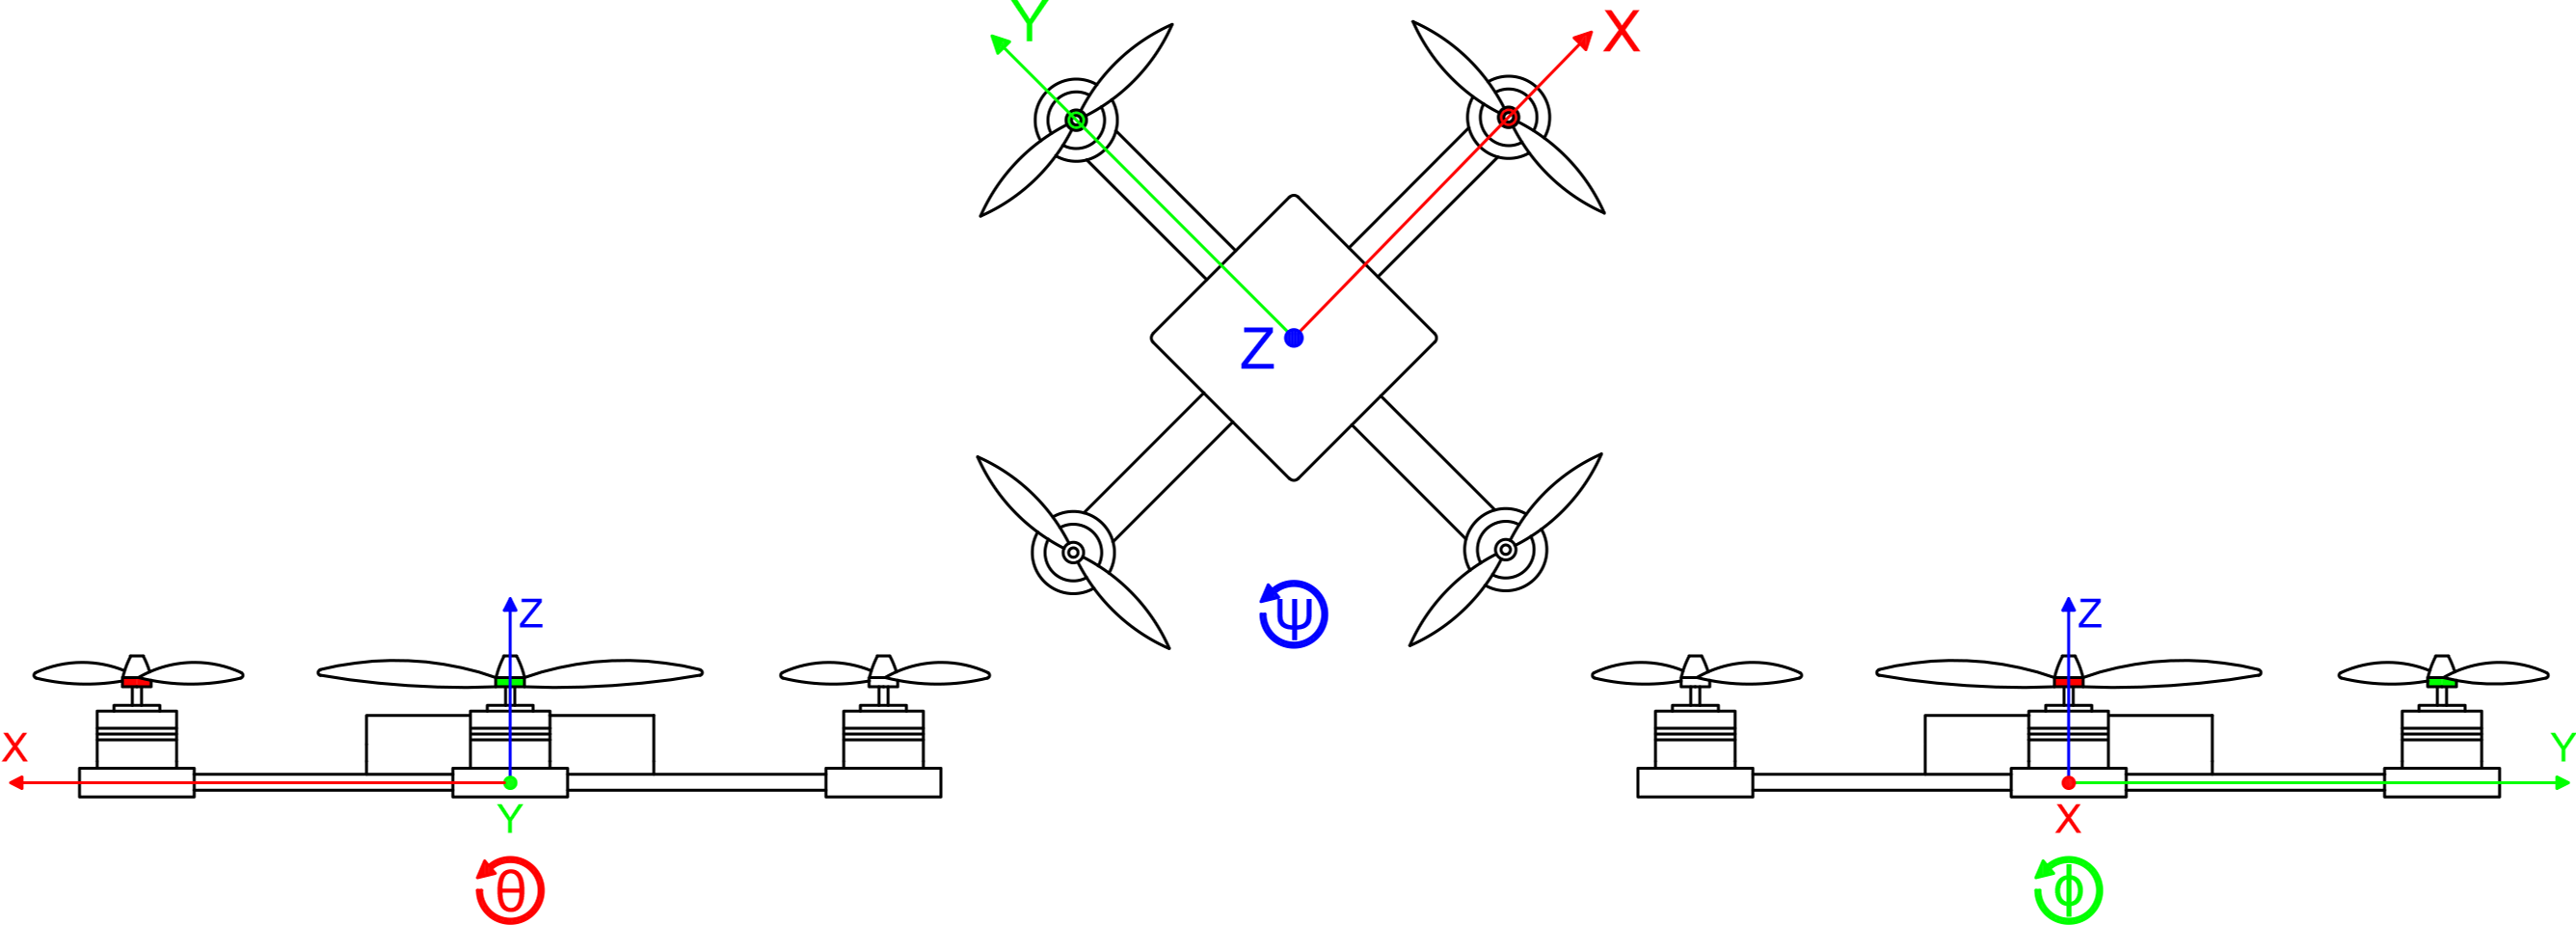
\includegraphics[width=1\textwidth]{capitulos/modelagem/imgs/drone_orientation.png}
    \label{fig:drone_orientations}
\end{figure}

As orientações estabelecidas pela Equação \ref{eq:atitude_escalar_som} são ilustradas na Figura \ref{fig:drone_orientations}. Para finalizar o equacionamento da dinâmica angular do sistema, os somatórios de momento podem ser descritos em termos dos momentos individuais de seus atuadores, ilustrados na Figura \ref{fig:attitude_dcl}. Substituindo tais torques na Equação \ref{eq:atitude_escalar_som} e denotando por $L$ a distância entre cada atuador e o centro da aeronave, a atitude do veículo é dada pela Equação \ref{eq:atitude_full}.

\begin{figure}[!h]
    \centering
    \caption{Diagrama de corpo livre da atitude de um quadricóptero com eixos orientados x, y e z em vermelho, verde e azul respectivamente além de forças e momentos em laranja.}
    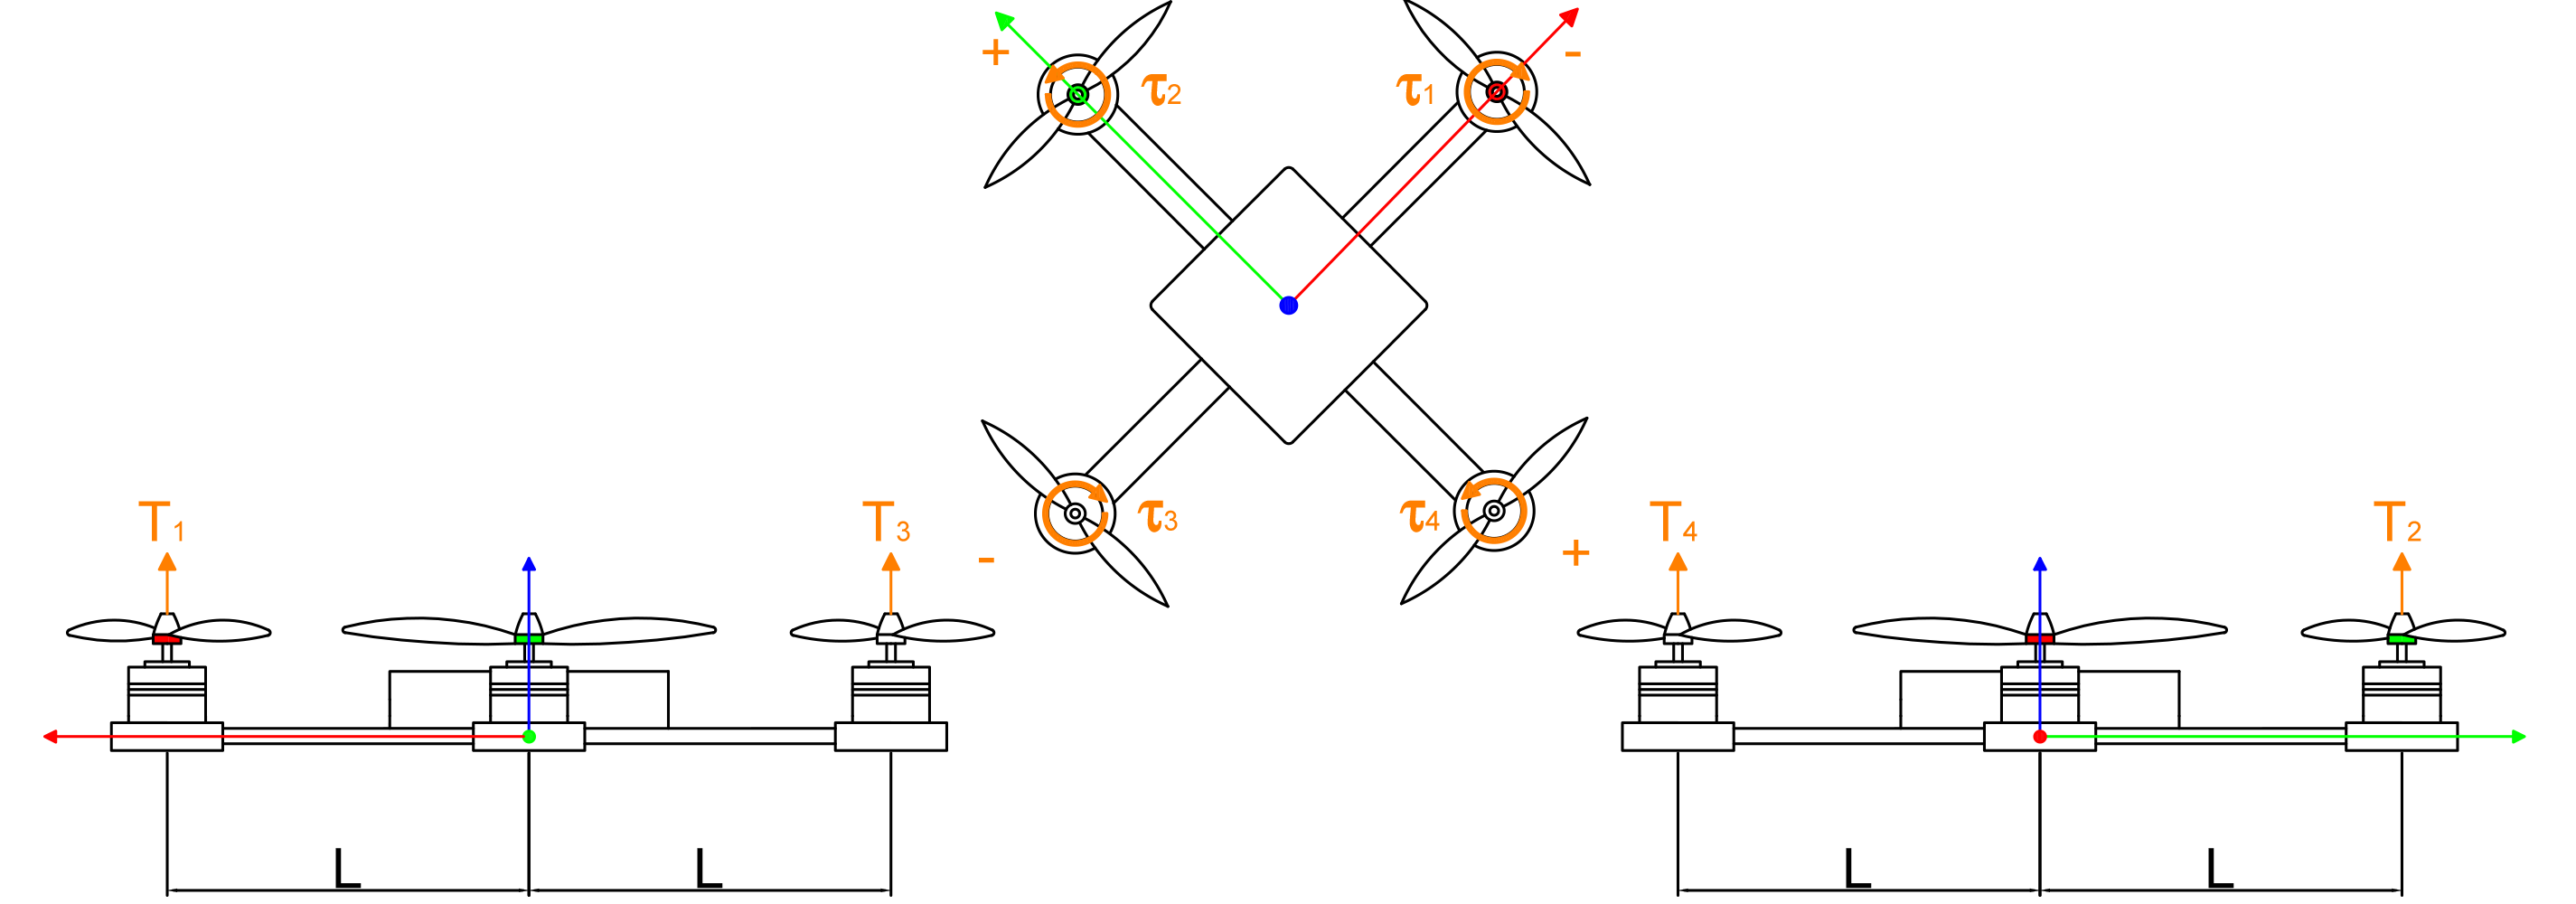
\includegraphics[width=1\textwidth]{capitulos/modelagem/imgs/attitude_dcl.png}
    \label{fig:attitude_dcl}
\end{figure}

\begin{equation}\label{eq:atitude_full}
    \begin{split}
        \dot{p} &= \frac{I_{zz} - I_{yy}}{I_{xx}}qr + \frac{I_r}{I_{xx}}\Omega q + \frac{L}{I_{xx}}(T_2 - T_4)\\
        \dot{q} &= \frac{I_{xx} - I_{zz}}{I_{yy}}pr - \frac{I_r}{I_{yy}}\Omega p + \frac{L}{I_{yy}}(T_1 - T_3)\\
        \dot{r} &= \frac{I_{yy} - I_{xx}}{I_{zz}}pq + \frac{-\tau_1 + \tau_2 - \tau_3 + \tau_4}{I_{zz}}
    \end{split}    
\end{equation}

Para descrever a translação do veículo, é preciso converter as coordenadas do sistema local para as de um global, conforme demonstrado pela Figura \ref{fig:ref_frame}. Este procedimento é realizado por meio da matriz de rotação da Equação \ref{eq:rotational_matrix_raw} \cite{robotica}, complementado pelo balanço de forças da Equação \ref{eq:translacao_vetor}, resultando na Equação \ref{eq:translacao:

\begin{figure}[!h]
    \centering
    \caption{Comparação da força dos propulsores no sistema de referências local X'Y'Z' para o sistema de referências global XYZ com eixos orientados x, y e z em vermelho, verde e azul respectivamente além da força em laranja.}
    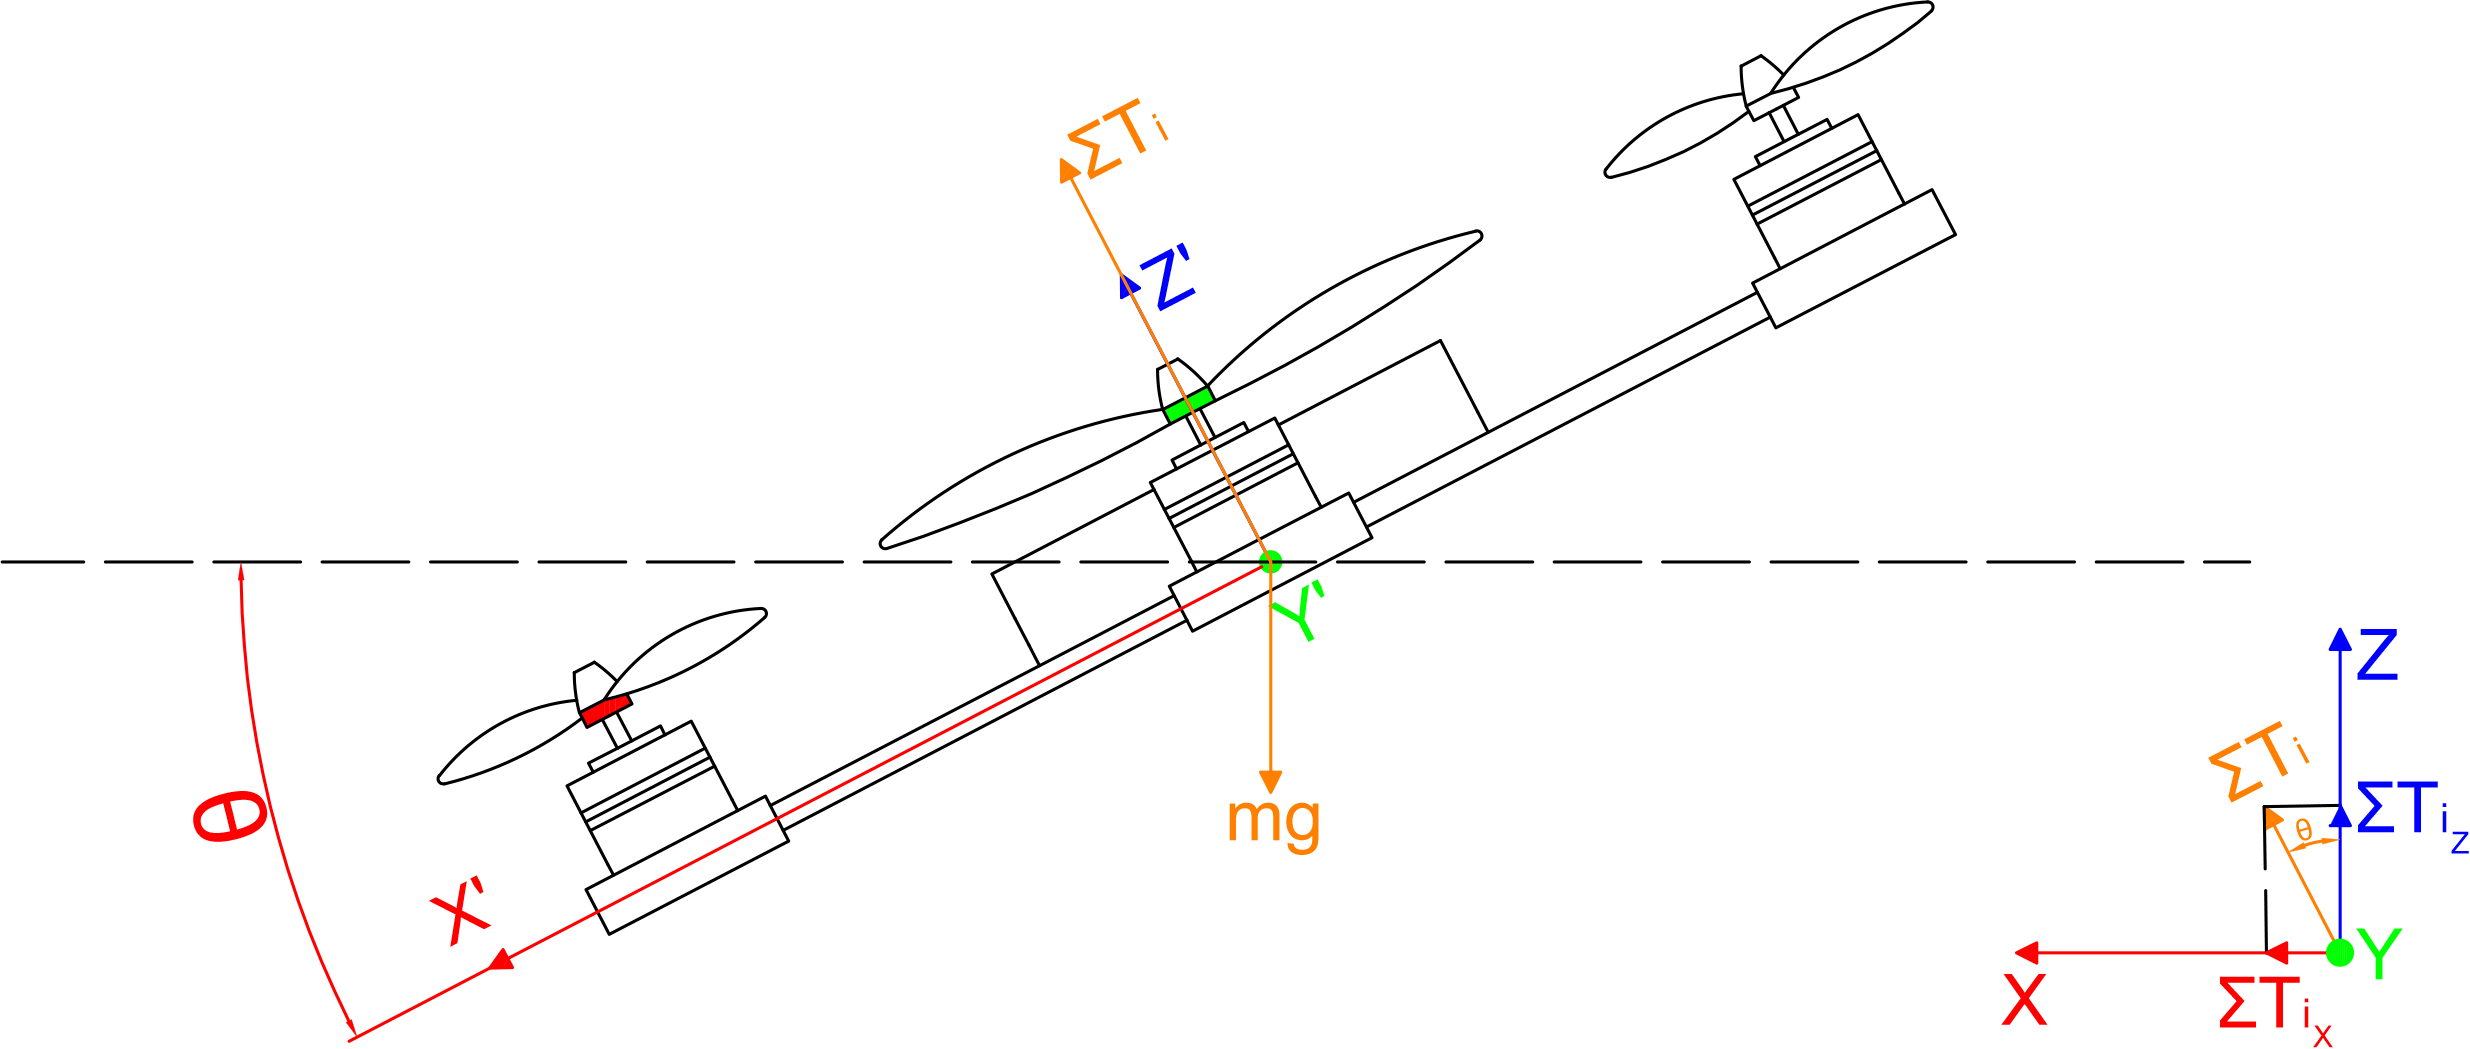
\includegraphics[width=0.85\textwidth]{capitulos/modelagem/imgs/ref_frame.png}
    \label{fig:ref_frame}
\end{figure}

\begin{equation}\label{eq:rotational_matrix_raw}
    \boldsymbol{R} = 
     \begin{bmatrix}
        \cos(\psi)  &   -\sin(\psi) &   0\\
        \sin(\psi)  &   \cos(\psi)  &   0\\
        0           &   0           &   1
    \end{bmatrix}_z
    \begin{bmatrix}
        \cos(\theta)    &   0             &   \sin(\theta)  \\
        0               &   1               &   0           \\
        -\sin(\theta)   &   0             &   \cos(\theta)
    \end{bmatrix}_y
   \begin{bmatrix}
        1           &   0           &   0               \\
        0           &   \cos(\phi)  &   -\sin(\phi)   \\
        0           &   \sin(\phi)  &   \cos(\phi)
    \end{bmatrix}_x
\end{equation}


\begin{equation}\label{eq:translacao_vetor}
    \begin{bmatrix}
        \Sigma F_x\\
        \Sigma F_y\\
        \Sigma F_z
    \end{bmatrix} 
    = m
    \begin{bmatrix}
        \ddot{z}\\
        \ddot{y}\\
        \ddot{z}
    \end{bmatrix} 
    = m
    \begin{bmatrix}
        0\\
        0\\
        -g
    \end{bmatrix}
    +
    R
    \begin{bmatrix}
        0\\
        0\\
        \Sigma T_i
    \end{bmatrix}_{local}
\end{equation}

\begin{equation}\label{eq:translacao}
    \begin{split}
        \ddot{x} &= (\sin{(\psi)}\sin{(\phi)} + \cos{(\psi)}\sin{(\theta)}\cos{(\phi)})\frac{\Sigma T_i}{m}\\
        \ddot{y} &= (-\cos{(\psi)}\sin{(\phi)} + \sin{(\psi)}\sin{(\theta)}\cos{(\phi)})\frac{\Sigma T_i}{m}\\
        \ddot{z} &= -g + \cos{(\theta)}\cos{(\phi)}\frac{\Sigma T_i}{m}
    \end{split}
\end{equation}

Finalmente, a dinâmica completa do movimento do quadricóptero é dada pelo uso combinado das equações que descrevem sua atitude com aquelas referentes à sua translação final, resultando:

\begin{equation}\label{eq:dinamica_raw}
    \begin{split}
        \ddot{x} &= (\sin{(\psi)}\sin{(\phi)} + \cos{(\psi)}\sin{(\theta)}\cos{(\phi)})\frac{\Sigma T_i}{m}\\
        \ddot{y} &= (-\cos{(\psi)}\sin{(\phi)} + \sin{(\psi)}\sin{(\theta)}\cos{(\phi)})\frac{\Sigma T_i}{m}\\
        \ddot{z} &= -g + \cos{(\theta)}\cos{(\phi)}\frac{\Sigma T_i}{m}\\
        \dot{p} &= \frac{I_{zz} - I_{yy}}{I_{xx}}qr + \frac{I_r}{I_{xx}}\Omega q + \frac{L}{I_{xx}}(T_2 - T_4)\\
        \dot{q} &= \frac{I_{xx} - I_{zz}}{I_{yy}}pr - \frac{I_r}{I_{yy}}\Omega p + \frac{L}{I_{yy}}(T_1 - T_3)\\
        \dot{r} &= \frac{I_{yy} - I_{xx}}{I_{zz}}pq + \frac{- \tau_1 + \tau_2 - \tau_3 + \tau_4}{I_{zz}}
    \end{split}
\end{equation}

\section{Simulação}

Para confirmar que modelagem ocorreu de maneira adequada e representa o sistema real de um quadricóptero, será utilizado um ambiente de simulação elaborado na ferramenta Simulink do \textit{software} MATLAB. O ambiente selecionado chama-se Quad-Sim, apresentado na Figura \ref{}, e foi desenvolvido por estudantes de Engenharia Mecânica da universidade de Drexel para um concurso elaborado pela IEEE.

\textcolor{red}{FOTO DO AMBIENTE DE SIMULAÇÃO}

O ambiente simula a dinâmica de um quadricóptero e permite um controle PID. Para este trabalho será utilizado apenas o bloco de \textit{Quadcopter Dynamics} e as visualizações 3D geradas pela GUI (\textit{Graphical User Interface}, ou Interface Gráfica do Usuário).

A fim de confirmar que o sistema modelado representa o mesmo sistema que o ambiente \textit{Quad-Sim} são efetuados diferentes testes que ocasionam a mudança da atitude do quadricóptero, os resultados são capturados na saída do bloco \textit{Quadcopter Dynamics} e na saída do bloco que representa a modelagem executada neste trabalho. Os resultados então são apresentados na Figura \ref{} com os parâmetros definidos na Tabela \ref{}.

\textcolor{red}{RESULTADOS GRÁFICOS}

% Aqui explicar que a gente vai usar um projeto matlab e comparar sinais com um projeto existente

% Explicar que no modelo foram usados diferentes numerações para os rotores, de forma que tem que mexer nos sinais

% Explicar que o modelo github utiliza a rotaçõa em pwm e tem que inverter as constantes de thrust e drag pra rad/s pra pensar igual ao meu

\end{document}